% Options for packages loaded elsewhere
\PassOptionsToPackage{unicode}{hyperref}
\PassOptionsToPackage{hyphens}{url}
\PassOptionsToPackage{dvipsnames,svgnames*,x11names*}{xcolor}
%
\documentclass[
]{memoir}
\usepackage{amsmath,amssymb}
\usepackage{lmodern}
\usepackage{ifxetex,ifluatex}
\ifnum 0\ifxetex 1\fi\ifluatex 1\fi=0 % if pdftex
  \usepackage[T1]{fontenc}
  \usepackage[utf8]{inputenc}
  \usepackage{textcomp} % provide euro and other symbols
\else % if luatex or xetex
  \usepackage{unicode-math}
  \defaultfontfeatures{Scale=MatchLowercase}
  \defaultfontfeatures[\rmfamily]{Ligatures=TeX,Scale=1}
  \setmonofont[]{Inconsolata}
\fi
% Use upquote if available, for straight quotes in verbatim environments
\IfFileExists{upquote.sty}{\usepackage{upquote}}{}
\IfFileExists{microtype.sty}{% use microtype if available
  \usepackage[]{microtype}
  \UseMicrotypeSet[protrusion]{basicmath} % disable protrusion for tt fonts
}{}
\makeatletter
\@ifundefined{KOMAClassName}{% if non-KOMA class
  \IfFileExists{parskip.sty}{%
    \usepackage{parskip}
  }{% else
    \setlength{\parindent}{0pt}
    \setlength{\parskip}{6pt plus 2pt minus 1pt}}
}{% if KOMA class
  \KOMAoptions{parskip=half}}
\makeatother
\usepackage{xcolor}
\IfFileExists{xurl.sty}{\usepackage{xurl}}{} % add URL line breaks if available
\IfFileExists{bookmark.sty}{\usepackage{bookmark}}{\usepackage{hyperref}}
\hypersetup{
  pdftitle={Data Science per psicologi},
  pdfauthor={Corrado Caudek},
  colorlinks=true,
  linkcolor=Maroon,
  filecolor=Maroon,
  citecolor=Blue,
  urlcolor=Blue,
  pdfcreator={LaTeX via pandoc}}
\urlstyle{same} % disable monospaced font for URLs
\usepackage{color}
\usepackage{fancyvrb}
\newcommand{\VerbBar}{|}
\newcommand{\VERB}{\Verb[commandchars=\\\{\}]}
\DefineVerbatimEnvironment{Highlighting}{Verbatim}{commandchars=\\\{\}}
% Add ',fontsize=\small' for more characters per line
\usepackage{framed}
\definecolor{shadecolor}{RGB}{248,248,248}
\newenvironment{Shaded}{\begin{snugshade}}{\end{snugshade}}
\newcommand{\AlertTok}[1]{\textcolor[rgb]{0.94,0.16,0.16}{#1}}
\newcommand{\AnnotationTok}[1]{\textcolor[rgb]{0.56,0.35,0.01}{\textbf{\textit{#1}}}}
\newcommand{\AttributeTok}[1]{\textcolor[rgb]{0.77,0.63,0.00}{#1}}
\newcommand{\BaseNTok}[1]{\textcolor[rgb]{0.00,0.00,0.81}{#1}}
\newcommand{\BuiltInTok}[1]{#1}
\newcommand{\CharTok}[1]{\textcolor[rgb]{0.31,0.60,0.02}{#1}}
\newcommand{\CommentTok}[1]{\textcolor[rgb]{0.56,0.35,0.01}{\textit{#1}}}
\newcommand{\CommentVarTok}[1]{\textcolor[rgb]{0.56,0.35,0.01}{\textbf{\textit{#1}}}}
\newcommand{\ConstantTok}[1]{\textcolor[rgb]{0.00,0.00,0.00}{#1}}
\newcommand{\ControlFlowTok}[1]{\textcolor[rgb]{0.13,0.29,0.53}{\textbf{#1}}}
\newcommand{\DataTypeTok}[1]{\textcolor[rgb]{0.13,0.29,0.53}{#1}}
\newcommand{\DecValTok}[1]{\textcolor[rgb]{0.00,0.00,0.81}{#1}}
\newcommand{\DocumentationTok}[1]{\textcolor[rgb]{0.56,0.35,0.01}{\textbf{\textit{#1}}}}
\newcommand{\ErrorTok}[1]{\textcolor[rgb]{0.64,0.00,0.00}{\textbf{#1}}}
\newcommand{\ExtensionTok}[1]{#1}
\newcommand{\FloatTok}[1]{\textcolor[rgb]{0.00,0.00,0.81}{#1}}
\newcommand{\FunctionTok}[1]{\textcolor[rgb]{0.00,0.00,0.00}{#1}}
\newcommand{\ImportTok}[1]{#1}
\newcommand{\InformationTok}[1]{\textcolor[rgb]{0.56,0.35,0.01}{\textbf{\textit{#1}}}}
\newcommand{\KeywordTok}[1]{\textcolor[rgb]{0.13,0.29,0.53}{\textbf{#1}}}
\newcommand{\NormalTok}[1]{#1}
\newcommand{\OperatorTok}[1]{\textcolor[rgb]{0.81,0.36,0.00}{\textbf{#1}}}
\newcommand{\OtherTok}[1]{\textcolor[rgb]{0.56,0.35,0.01}{#1}}
\newcommand{\PreprocessorTok}[1]{\textcolor[rgb]{0.56,0.35,0.01}{\textit{#1}}}
\newcommand{\RegionMarkerTok}[1]{#1}
\newcommand{\SpecialCharTok}[1]{\textcolor[rgb]{0.00,0.00,0.00}{#1}}
\newcommand{\SpecialStringTok}[1]{\textcolor[rgb]{0.31,0.60,0.02}{#1}}
\newcommand{\StringTok}[1]{\textcolor[rgb]{0.31,0.60,0.02}{#1}}
\newcommand{\VariableTok}[1]{\textcolor[rgb]{0.00,0.00,0.00}{#1}}
\newcommand{\VerbatimStringTok}[1]{\textcolor[rgb]{0.31,0.60,0.02}{#1}}
\newcommand{\WarningTok}[1]{\textcolor[rgb]{0.56,0.35,0.01}{\textbf{\textit{#1}}}}
\usepackage{longtable,booktabs,array}
\usepackage{calc} % for calculating minipage widths
% Correct order of tables after \paragraph or \subparagraph
\usepackage{etoolbox}
\makeatletter
\patchcmd\longtable{\par}{\if@noskipsec\mbox{}\fi\par}{}{}
\makeatother
% Allow footnotes in longtable head/foot
\IfFileExists{footnotehyper.sty}{\usepackage{footnotehyper}}{\usepackage{footnote}}
\makesavenoteenv{longtable}
\usepackage{graphicx}
\makeatletter
\def\maxwidth{\ifdim\Gin@nat@width>\linewidth\linewidth\else\Gin@nat@width\fi}
\def\maxheight{\ifdim\Gin@nat@height>\textheight\textheight\else\Gin@nat@height\fi}
\makeatother
% Scale images if necessary, so that they will not overflow the page
% margins by default, and it is still possible to overwrite the defaults
% using explicit options in \includegraphics[width, height, ...]{}
\setkeys{Gin}{width=\maxwidth,height=\maxheight,keepaspectratio}
% Set default figure placement to htbp
\makeatletter
\def\fps@figure{htbp}
\makeatother
\setlength{\emergencystretch}{3em} % prevent overfull lines
\providecommand{\tightlist}{%
  \setlength{\itemsep}{0pt}\setlength{\parskip}{0pt}}
\setcounter{secnumdepth}{5}
\chapterstyle{bianchi}

\usepackage{amsmath}
\usepackage[italian]{babel} 
\usepackage{lmodern} 
\usepackage{booktabs}
\usepackage{hyperref}
\hypersetup{
  colorlinks=true
}
\usepackage[
  labelfont=bf, 
  font={small, it} 
]{caption} 
\usepackage{upquote} % print correct quotes in verbatim-environments
\usepackage[autostyle, italian=quotes]{csquotes}
\usepackage{xfrac}

\raggedbottom % allow variable (ragged) site heights
\frenchspacing
\setlength\parskip{1.5pt plus 1pt minus 0.5pt}

\DeclareMathOperator{\Var}{Var} % Define variance operator
\DeclareMathOperator{\SD}{SD} % Define sd operator
\DeclareMathOperator{\Cov}{Cov} % Define covariance operator
\DeclareMathOperator{\Corr}{Corr} % Define correlation operator
\DeclareMathOperator{\Me}{Me} % Define mediane operator
\DeclareMathOperator{\Mo}{Mo} % Define mode operator
\DeclareMathOperator{\Bin}{Bin} % Define binomial operator
\DeclareMathOperator{\Cauchy}{Cauchy} % Define Cauchy operator
\DeclareMathOperator{\Beta}{Beta} % Define Beta operator
\DeclareMathOperator{\B}{\mathscr{B}} % Define Bernoulli operator
\newcommand{\R}{\textsf{R}} % Define R programming language symbol
\newcommand{\E}{\mathbb{E}} % Define expected value operator
\newcommand{\Real}{\mathbb{R}} % Define real number operator
\newcommand{\Prob}{\mathscr{P}}
\DeclareMathOperator*{\argmin}{arg\,min} % thin space, limits on side in displays
\DeclareMathOperator*{\argmax}{arg\,max} % thin space, limits on side in displays

\usepackage{microtype}

\ifluatex
  \usepackage{selnolig}  % disable illegal ligatures
\fi
\usepackage[]{natbib}
\bibliographystyle{apalike}

\title{Data Science per psicologi}
\author{Corrado Caudek}
\date{2021-09-13}

\usepackage{amsthm}
\newtheorem{theorem}{Teorema}[chapter]
\newtheorem{lemma}{Lemma}[chapter]
\newtheorem{corollary}{Corollario}[chapter]
\newtheorem{proposition}{Proposizione}[chapter]
\newtheorem{conjecture}{Congettura}[chapter]
\theoremstyle{definition}
\newtheorem{definition}{Definizione}[chapter]
\theoremstyle{definition}
\newtheorem{example}{Esempio}[chapter]
\theoremstyle{definition}
\newtheorem{exercise}{Exercizio}[chapter]
\theoremstyle{definition}
\newtheorem{hypothesis}{Hypothesis}[chapter]
\theoremstyle{remark}
\newtheorem*{remark}{Osservazione}
\newtheorem*{solution}{Soluzione}
\begin{document}
\maketitle

{
\hypersetup{linkcolor=}
\setcounter{tocdepth}{1}
\tableofcontents
}
\newpage

\vspace*{5cm}

\thispagestyle{empty}

\hypertarget{chapter-distr-coniugate}{%
\chapter{Distribuzioni a priori coniugate}\label{chapter-distr-coniugate}}

\hypertarget{il-denominatore-bayesiano}{%
\section{Il denominatore bayesiano}\label{il-denominatore-bayesiano}}

In generale, in un problema bayesiano i dati \(y\) provengono da una densità \(p(y \mid \theta)\) e al parametro \(\theta\) viene assegnata una densità a priori \(p(\theta)\). La scelta della distribuzione a priori per i parametri è l'aspetto cruciale dell'impostazione bayesiana in quanto la distribuzione a priori è lo strumento attraverso cui le informazioni extra-sperimentali vengono inserite nel procedimento induttivo. La scelta della distribuzione a priori che meglio rappresenta le credenze iniziali implica che agenti diversi possono specificare sia le stesse distribuzioni di probabilità ma con diversi valori dei parametri, sia diverse distribuzioni di probabilità. Da ciò deriva una componente soggettiva. La scelta della distribuzione a priori ha inoltre importanti conseguenze di tipo computazionale. A meno di non utilizzare particolari forme analitiche, in generale risulta impossibile ottenere espressioni analitiche in forma esplicita per le distribuzioni a posteriori. Ciò dipende dal denominatore del rapporto di Bayes.

Dopo che un campione \(Y = y\) è stato osservato, la funzione di verosimiglianza è uguale a \(\mathcal{L}(\theta) = p(y \mid \theta)\) e la densità a posteriori è

\[
p(\theta \mid y) = \frac{p(\theta) p(y \mid \theta)}{\int p(\theta) p(y \mid \theta) d \theta}.
\]
Si noti che al denominatore troviamo un integrale. Tale integrale può essere risolto per via analitica solo se vengono usate le cosiddette \emph{distribuzioni a priori coniugate per la verosimiglianza}.

Inoltre, i sommari della distribuzione a posteriori sono espressi come rapporto di integrali. Ad esempio, la media a posteriori di \(\theta\) è data da

\[
\E(\theta \mid y) = \frac{\int \theta \pi(\theta) p(y \mid \theta) d \theta}{\int \pi(\theta) p(y \mid \theta) d \theta}.
\]
Il calcolo del valore atteso a posteriori richiede dunque la valutazione di due integrali, ciascuno dei quali non esprimibile in forma chiusa.

Per questa ragione, la strada principale che viene seguita nella modellistica bayesiana è quella che porta a determinare la distribuzione a posteriori non per via analitica, ma bensì mediante metodi numerici. La simulazione fornisce dunque la strategia generale del calcolo bayesiano. A questo fine vengono usati i metodi di campionamento detti Monte-Carlo Markov-Chain (MCMC). Tali metodi costituiscono una potente e praticabile alternativa per la costruzione della distribuzione a posteriori per modelli complessi e consentono di decidere quali distribuzioni a priori e quali distribuzioni di verosimiglianza usare sulla base di considerazioni teoriche soltanto, senza dovere preoccuparsi di altri vincoli. Dato che è basata su metodi computazionalmente intensivi, la stima numerica della funzione a posteriori può essere svolta soltanto mediante software. In anni recenti i metodi bayesiani di analisi dei dati sono diventati sempre più popolari proprio perché la potenza di calcolo necessaria per svolgere tali calcoli è ora alla portata di tutti. Questo non era vero solo pochi decenni fa.

\hypertarget{le-distribuzioni-coniugate}{%
\section{Le distribuzioni coniugate}\label{le-distribuzioni-coniugate}}

Una distribuzione di probabilità a priori si dice coniugata al modello utilizzato se appartiene alla stessa classe di distribuzioni della distribuzione a posteriori; in tali circostanze la distribuzione a priori e la distribuzione a posteriori differiscono solo per il valore dei parametri.

\begin{definition}
Sia data la funzione di verosimiglianza \(p(\theta \mid y)\) e sia \(\mathcal{D}\) una classe di densità a priori per \(\theta\). La famiglia di distribuzioni a priori \(\mathcal{D}\) è coniugata al modello se avviene che

\[
p(\theta \mid y) \in \mathcal{D}.
\]

\noindent
Pertanto ciò che cambia nella distribuzione a posteriori non è la forma della distribuzione ma solo i parametri.
\end{definition}

L'uso di distribuzioni a priori coniugate consente di determinare la distribuzione a posteriori per via analitica. Per quanto ``semplice'' in termini formali, questo approccio, però, limita di molto le possibili scelte del ricercatore. Nel senso che non è sempre sensato, dal punto di vista teorico, utilizzare distribuzioni a priori coniugate per la verosimiglianza per i parametri di interesse.
Detto in altre parole: è possibile ottenere la distribuzione posteriore per via analitica solo per alcune specifiche combinazioni di distribuzione a priori e verosimiglianza, ma questo limita considerevolmente la flessibilità della modellizzazione.

\hypertarget{chapter-distr-priori-coniugate}{%
\section{Il modello Beta-Binomiale}\label{chapter-distr-priori-coniugate}}

Obiettivo di questo Capitolo è mostrare come sia possibile calcolare in maniera esatta la distribuzione a posteriori mediante l'uso di una distribuzione a priori coniugata. Esamineremo qui il caso più semplice, ovvero quello Beta-Binomiale.

Per fare un esempio concreto, verranno qui considerati i dati di \citet{zetschefuture2019}. Questi ricercatori si sono chiesti se gli individui depressi manifestino delle aspettative accurate circa il loro umore futuro, oppure se tali aspettative risultino distorte negativamente. Nell'esempio considereremo i 30 partecipanti dello studio di \citet{zetschefuture2019} che hanno riportato la presenza di un episodio di depressione maggiore in atto. All'inizio della settimana di test, a questi pazienti è stato chiesto di valutare l'umore che si aspettavano di esperire nei giorni seguenti della settimana. Mediante una app, i partecipanti dovevano poi valutare il proprio umore in cinque momenti diversi di cinque giorni successivi. Lo studio prende in esame diverse emozioni, ma qui ci concentreremo unicamente sulla tristezza.

Utilizzando i dati forniti dagli autori, è stata calcolata la media dei giudizi relativi al livello di tristezza raccolti da ciascun partecipante tramite la app. Tale media è stata poi sottratta dall'aspettativa del livello di tristezza fornita all'inizio della settimana. La discrepanza tra aspettative e realtà è stata considerata come un evento dicotomico: valori positivi di tale differenza indicano che le aspettative circa il livello di tristezza erano maggiori del livello di tristezza effettivamente esperito --- ciò significa che le aspettative future risultano negativamente distorte (evento codificato con ``1''). Viceversa, si ha che le aspettative risultano positivamente distorte se la differenza descritta in precedenza assume un valore negativo (evento codificato con ``0''). Nel campione dei 30 partecipanti clinici di \citet{zetschefuture2019}, le aspettative future di 23 partecipanti risultano distorte negativamente e quelle di 7 partecipanti risultano distorte positivamente.

Nel seguito, indicherò con \(\theta\) la probabilità che le aspettative del partecipante siano distorte negativamente (ovvero, la probabilità dell'evento codificato con ``1''). Il problema dell'esercizio è quello di ottenere la stima a posteriori di \(\theta\) alla luce dei dati corrispondenti a 23 ``successi'' in 30 prove.\footnote{Si noti un punto importante: dire semplicemente che la stima di \(\theta\) è uguale a 23/30 = 0.77 ci porta ad ignorare il livello di incertezza associato a tale stima. Infatti, lo stesso valore (0.77) si può ottenere come 23/30, o 230/300, o 2300/3000, o 23000/30000, ma l'incertezza di una stima pari a 0.77 è molto diversa nei quattro casi. Quando si traggono conclusioni dai dati è invece necessario quantificare il livello della nostra incertezza relativamente alla stima del parametro di interesse (nel caso presente, \(\theta\)). Lo strumento ci consente di quantificare tale incertezza è la distribizione a posteriori \(p(\theta \mid y)\). Ovviamente, \(p(\theta \mid y)\) assume forme molto diverse nei quattro casi descritti sopra.}

Nel caso presente, i dati (23 ``successi'' in 30 prove) possono essere considerati come realizzazioni indipendenti di una variabile casuale Bernoulliana. In tali circostanze, esiste una famiglia di distribuzioni che, qualora venga scelta per la distribuzione a priori, fa sì che la distribuzione a posteriori abbia la stessa forma funzionale della distribuzione a priori. Questo consente una soluzione analitica dell'integrale che compare nel denominatore bayesiano. Nel caso del modello binomiale, la famiglia di distribuzioni che ha questa proprietà è la distribuzione Beta.

\hypertarget{parametri-della-distribuzione-beta}{%
\subsection{Parametri della distribuzione Beta}\label{parametri-della-distribuzione-beta}}

Usando la distribuzione Beta è possibile esprimere diverse credenze iniziali rispetto a \(\theta\). Scegliere \(a=4\) e \(b=4\) per la distribuzione a priori Beta significa dire che, prima di avere esaminato i dati, una ``aspettativa futura distorta negativamente'' è tanto probabile quanto una ``aspettativa futura non distorta negativamente''; tuttavia, ad una tale proposizione è associato un livello di certezza piuttosto basso. Possiamo esprimere la nostra incertezza calcolando, con un grado di fiducia del 95\%, la regione nella quale, in base a tale ipotesi a priori, si trova il valore del parametro. Per ottenere tale intervallo di credibilità a priori, usiamo la funzione \texttt{qbeta()} di \(\R\). In \texttt{qbeta()} i parametri \(a\) e \(b\) sono chiamati \texttt{shape1} e \texttt{shape2}:

\begin{Shaded}
\begin{Highlighting}[]
\FunctionTok{qbeta}\NormalTok{(}\FunctionTok{c}\NormalTok{(}\FloatTok{0.025}\NormalTok{, }\FloatTok{0.975}\NormalTok{), }\AttributeTok{shape1 =} \DecValTok{4}\NormalTok{, }\AttributeTok{shape2 =} \DecValTok{4}\NormalTok{)}
\CommentTok{\#\textgreater{} [1] 0.1840516 0.8159484}
\end{Highlighting}
\end{Shaded}

Se scegliamo \(a=10\) e \(b=10\) supponiamo ancora a priori che una ``aspettativa futura distorta negativamente'' sia altrettanto probabile di una ``aspettativa futura non distorta negativamente'', ma ora la nostra certezza a priori sul valore del parametro è maggiore, come indicato dall'intervallo al 95\%:

\begin{Shaded}
\begin{Highlighting}[]
\FunctionTok{qbeta}\NormalTok{(}\FunctionTok{c}\NormalTok{(}\FloatTok{0.025}\NormalTok{, }\FloatTok{0.975}\NormalTok{), }\AttributeTok{shape1 =} \DecValTok{10}\NormalTok{, }\AttributeTok{shape2 =} \DecValTok{10}\NormalTok{)}
\CommentTok{\#\textgreater{} [1] 0.2886432 0.7113568}
\end{Highlighting}
\end{Shaded}

Quale distribuzione a priori dobbiamo scegliere? In un problema concreto di analisi dei dati, la scelta della distribuzione a priori dipende da quali sono le credenze a priori vogliamo includere nell'analisi dei dati. Se non abbiamo alcuna informazione a priori, potremmo usare \(a=1\) e \(b=1\), il che produce una distribuzione a priori uniforme. Questa, tuttavia, è una cattiva idea, se pensiamo al problema della riparametrizzazione. In tali circostanze è invece raccomandato usare una distribuzione a priori vagamente informativa, come \(\text{Beta}(2, 2)\).

Nella successiva discussione, per fare un esempio, useremo una \(\text{Beta}(2, 10)\) quale distribuzione a priori, ovvero:

\[
p(\theta) = \frac{\Gamma(12)}{\Gamma(2)\Gamma(10)}\theta^{2-1} (1-\theta)^{10-1}.
\]

\hypertarget{la-specificazione-della-distribuzione-a-posteriori}{%
\subsection{La specificazione della distribuzione a posteriori}\label{la-specificazione-della-distribuzione-a-posteriori}}

Una volta scelta la distribuzione a priori di tipo Beta, i cui parametri rispecchiano il giudizio a priori di probabilità, la distribuzione a posteriori viene specificata dalla regola di Bayes:

\[
\text{distribuzione a posteriori} = \frac{\text{verosimiglianza}\cdot\text{distribuzione a priori}}{\text{verosimiglianza marginale}}.
\]

Nel caso presente abbiamo

\[
p(\theta \mid n=30, y=23) = \frac{\Big[\binom{30}{23}\theta^{23}(1-\theta)^{30-23}\Big]\Big[\frac{\Gamma(12)}{\Gamma(2)\Gamma(10)}\theta^{2-1} (1-\theta)^{10-1}\Big]}{p(y = 23)},
\]
\noindent
laddove \(p(y = 23)\) è \(\int_0^1p(y = 23 \mid n = 30, \theta)\). Questo termine, ovvero la verosimiglianza marginale, è una costante di normalizzazione che fa sì che l'area sottesa alla densità a posteriori sia unitaria.

Raccogliendo tutte le costanti dell'equazione precedente ottiamo

\[
p(\theta \mid n=30, y=23) =\left[\frac{\binom{30}{23}\frac{\Gamma(12)}{\Gamma(2)\Gamma(10)}}{p(y = 23)}\right] \theta^{23}(1-\theta)^{7}\theta^{1} (1-\theta)^{9}.
\]

Se ignoriamo il termine costante all'interno della parentesi quadra abbiamo:

\begin{align}
p(\theta \mid n=30, y=23) &\propto \theta^{23}(1-\theta)^{7}\theta^{1} (1-\theta)^{9}\notag\\
&\propto \theta^{24}(1-\theta)^{16}.\notag
\end{align}

Il termine di destra dell'equazione precedente corrisponde ad una distribuzione Beta di parametri \(\alpha=25\) e \(\beta = 17\). Il risultato così ottenuto individua il \emph{kernel} della distribuzione a posteriori, ovvero la distribuzione a posteriori non normalizzata. Infatti, l'area sotto la curva (AUC)

\begin{Shaded}
\begin{Highlighting}[]
\NormalTok{postFun }\OtherTok{\textless{}{-}} \ControlFlowTok{function}\NormalTok{(theta) \{}
\NormalTok{  theta}\SpecialCharTok{\^{}}\DecValTok{24} \SpecialCharTok{*}\NormalTok{ (}\DecValTok{1} \SpecialCharTok{{-}}\NormalTok{ theta)}\SpecialCharTok{\^{}}\DecValTok{16}
\NormalTok{\}}
\NormalTok{(AUC }\OtherTok{\textless{}{-}} \FunctionTok{integrate}\NormalTok{(postFun, }\AttributeTok{lower =} \DecValTok{0}\NormalTok{, }\AttributeTok{upper =} \DecValTok{1}\NormalTok{)}\SpecialCharTok{$}\NormalTok{value)}
\CommentTok{\#\textgreater{} [1] 3.880577e{-}13}
\end{Highlighting}
\end{Shaded}

\noindent
non è 1. Per ottenere una corretta distribuzione di densità è necessario includere una costante di normalizzazione. In base alla definizione della distribuzione Beta, tale costante è

\[
\frac{\Gamma(a+b)}{\Gamma(a)\Gamma(b)} = \frac{\Gamma(42)}{\Gamma(25)\Gamma(17)}.
\]
Questo termine non è altro che l'integrale della distribuzione a posteriori non normalizzata che è stato calcolato in precedenza:

\begin{Shaded}
\begin{Highlighting}[]
\NormalTok{postFun }\OtherTok{\textless{}{-}} \ControlFlowTok{function}\NormalTok{(theta) \{}
\NormalTok{  theta}\SpecialCharTok{\^{}}\DecValTok{24} \SpecialCharTok{*}\NormalTok{ (}\DecValTok{1} \SpecialCharTok{{-}}\NormalTok{ theta)}\SpecialCharTok{\^{}}\DecValTok{16} \SpecialCharTok{/}\NormalTok{ AUC}
\NormalTok{\}}
\FunctionTok{integrate}\NormalTok{(postFun, }\AttributeTok{lower =} \DecValTok{0}\NormalTok{, }\AttributeTok{upper =} \DecValTok{1}\NormalTok{)}\SpecialCharTok{$}\NormalTok{value}
\CommentTok{\#\textgreater{} [1] 1}
\end{Highlighting}
\end{Shaded}

\noindent
Infatti, l'area sottesa alla funzione

\[
p(\theta \mid n=30, y=23) =  \frac{\Gamma(42)}{\Gamma(25)\Gamma(17)}\theta^{25-1}(1-\theta)^{17-1} = \text{Beta}(y+a, n-y+b)
\]
\noindent
somma ad 1, ovvero,

\begin{Shaded}
\begin{Highlighting}[]
\NormalTok{postFunNor }\OtherTok{\textless{}{-}} \ControlFlowTok{function}\NormalTok{(theta) \{}
\NormalTok{  (}\FunctionTok{factorial}\NormalTok{(}\DecValTok{42{-}1}\NormalTok{) }\SpecialCharTok{/}\NormalTok{ (}\FunctionTok{factorial}\NormalTok{(}\DecValTok{25{-}1}\NormalTok{)}\SpecialCharTok{*}\FunctionTok{factorial}\NormalTok{(}\DecValTok{17{-}1}\NormalTok{))) }\SpecialCharTok{*} 
\NormalTok{    theta}\SpecialCharTok{\^{}}\NormalTok{(}\DecValTok{25{-}1}\NormalTok{) }\SpecialCharTok{*}\NormalTok{ (}\DecValTok{1} \SpecialCharTok{{-}}\NormalTok{ theta)}\SpecialCharTok{\^{}}\NormalTok{(}\DecValTok{17{-}1}\NormalTok{)}
\NormalTok{\}}
\NormalTok{(AUC2 }\OtherTok{\textless{}{-}} \FunctionTok{integrate}\NormalTok{(postFunNor, }\AttributeTok{lower =} \DecValTok{0}\NormalTok{, }\AttributeTok{upper =} \DecValTok{1}\NormalTok{)}\SpecialCharTok{$}\NormalTok{value)}
\CommentTok{\#\textgreater{} [1] 1}
\end{Highlighting}
\end{Shaded}

Possiamo quindi riassumere dicendo che siamo partiti da una verosimiglianza \(\Bin(n = 30, y = 23 \mid \theta)\) e, moltiplicando la verosimiglianza per la distribuzione a priori \(\theta \sim \text{Beta}(2, 10)\), abbiamo ottenuto la distribuzione a posteriori \(p(\theta \mid n, y) \sim \text{Beta}(25, 17)\). Questo è un esempio di analisi coniugata: la distribuzione a posteriori del parametro ha la stessa forma funzionale della distribuzione a priori. La presente combinazione di verosimiglianza e distribuzione a priori è chiamata caso coniugato \emph{Beta-Binomiale} ed è descritto dal seguente teorema.

\begin{theorem}
\protect\hypertarget{thm:beta-binom}{}\label{thm:beta-binom}Sia data la funzione di verosimiglianza \(\Bin(n, y \mid \theta)\) e sia \(\text{Beta}(\alpha, \beta)\) una distribuzione a priori. In tali circostanze, la distribuzione a posteriori del parametro \(\theta\) sarà una distribuzione \(\text{Beta}(\alpha + y, \beta + n - y)\).
\end{theorem}

\noindent
In particolare, possiamo calcolare qual è il valore atteso a posteriori di \(\theta\). Essendo \(\E[\text{Beta}(\alpha, \beta)] = \frac{\alpha}{\alpha + \beta}\), il valore atteso a posteriori di \(\theta\) sarà

\begin{equation}
\E_{\text{post}} [\Beta(\alpha + y, \beta + n - y)] = \frac{\alpha + y}{\alpha + \beta +n}.
\label{eq:ev-post-beta-bin-1}
\end{equation}

\begin{example}

Per i dati esaminati, usando la \ref{thm:beta-binom} possiamo ottenere l'intervallo di credibilità a posteriori del 95\% per il parametro \(\theta\) come:

\begin{Shaded}
\begin{Highlighting}[]
\FunctionTok{qbeta}\NormalTok{(}\FunctionTok{c}\NormalTok{(}\FloatTok{0.025}\NormalTok{, }\FloatTok{0.975}\NormalTok{), }\AttributeTok{shape1 =} \DecValTok{25}\NormalTok{, }\AttributeTok{shape2 =} \DecValTok{17}\NormalTok{)}
\CommentTok{\#\textgreater{} [1] 0.4450478 0.7368320}
\end{Highlighting}
\end{Shaded}

La media della distribuzione a posteriori è

\begin{Shaded}
\begin{Highlighting}[]
\DecValTok{25} \SpecialCharTok{/}\NormalTok{ (}\DecValTok{25} \SpecialCharTok{+} \DecValTok{17}\NormalTok{)}
\CommentTok{\#\textgreater{} [1] 0.5952381}
\end{Highlighting}
\end{Shaded}

La moda della distribuzione a posteriori è

\begin{Shaded}
\begin{Highlighting}[]
\NormalTok{(}\DecValTok{25} \SpecialCharTok{{-}} \DecValTok{1}\NormalTok{) }\SpecialCharTok{/}\NormalTok{ (}\DecValTok{25} \SpecialCharTok{+} \DecValTok{17} \SpecialCharTok{{-}} \DecValTok{2}\NormalTok{)}
\CommentTok{\#\textgreater{} [1] 0.6}
\end{Highlighting}
\end{Shaded}

La deviazione standard della distribuzione a priori è

\begin{Shaded}
\begin{Highlighting}[]
\FunctionTok{sqrt}\NormalTok{((}\DecValTok{25} \SpecialCharTok{*} \DecValTok{17}\NormalTok{) }\SpecialCharTok{/}\NormalTok{ ((}\DecValTok{25} \SpecialCharTok{+} \DecValTok{17}\NormalTok{)}\SpecialCharTok{\^{}}\DecValTok{2} \SpecialCharTok{*}\NormalTok{ (}\DecValTok{25} \SpecialCharTok{+} \DecValTok{17} \SpecialCharTok{+} \DecValTok{1}\NormalTok{)))}
\CommentTok{\#\textgreater{} [1] 0.0748533}
\end{Highlighting}
\end{Shaded}

\end{example}

\begin{example}

La funzione R \texttt{plot\_beta\_binomial()} del pacchetto \texttt{bayesrules} descrive in maniera grafica l'aggiornamento bayesiano Beta-Binomiale:

\begin{Shaded}
\begin{Highlighting}[]
\NormalTok{bayesrules}\SpecialCharTok{::}\FunctionTok{plot\_beta\_binomial}\NormalTok{(}
  \AttributeTok{alpha =} \DecValTok{2}\NormalTok{, }\AttributeTok{beta =} \DecValTok{10}\NormalTok{, }\AttributeTok{y =} \DecValTok{23}\NormalTok{, }\AttributeTok{n =} \DecValTok{30}
\NormalTok{)}
\end{Highlighting}
\end{Shaded}

\begin{center}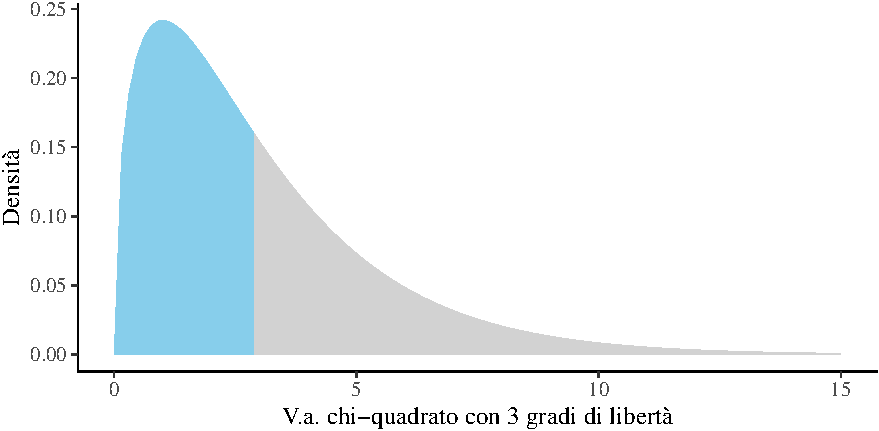
\includegraphics{026_distr_coniugate_files/figure-latex/unnamed-chunk-10-1} \end{center}

Un sommario delle distribuzioni a priori e a posteriori si ottiene usando la funzione \texttt{summarize\_beta\_binomial()}:

\begin{Shaded}
\begin{Highlighting}[]
\NormalTok{bayesrules}\SpecialCharTok{:::}\FunctionTok{summarize\_beta\_binomial}\NormalTok{(}
  \AttributeTok{alpha =} \DecValTok{2}\NormalTok{, }\AttributeTok{beta =} \DecValTok{10}\NormalTok{, }\AttributeTok{y =} \DecValTok{23}\NormalTok{, }\AttributeTok{n =} \DecValTok{30}
\NormalTok{)}
\CommentTok{\#\textgreater{}       model alpha beta      mean mode         var        sd}
\CommentTok{\#\textgreater{} 1     prior     2   10 0.1666667  0.1 0.010683761 0.1033623}
\CommentTok{\#\textgreater{} 2 posterior    25   17 0.5952381  0.6 0.005603016 0.0748533}
\end{Highlighting}
\end{Shaded}

\end{example}

\begin{example}

Consideriamo un altro esempio discusso da \citet{Johnson2022bayesrules}. Nel 1963, Stanley Milgram presentò una ricerca sulla propensione delle persone a obbedire agli ordini di figure di autorità, anche quando tali ordini possono danneggiare altre persone \citep{milgram1963behavioral}. Nell'articolo, Milgram descrive lo studio come

\begin{quote}
consist{[}ing{]} of ordering a naive subject to administer electric shock to a victim. A simulated shock generator is used, with 30 clearly marked voltage levels that range from IS to 450 volts. The instrument bears verbal designations that range from Slight Shock to Danger: Severe Shock. The responses of the victim, who is a trained confederate of the experimenter, are standardized. The orders to administer shocks are given to the naive subject in the context of a `learning experiment' ostensibly set up to study the effects of punishment on memory. As the experiment proceeds the naive subject is commanded to administer increasingly more intense shocks to the victim, even to the point of reaching the level marked Danger: Severe Shock.
\end{quote}

All'insaputa del partecipante, gli shock elettrici erano falsi e l'attore stava solo fingendo di provare il dolore dello shock.

\citet{Johnson2022bayesrules} fanno inferenza sui risultati dello studio di Milgram mediante il modello Beta-Binomiale. Il parametro di interesse è \(\theta\), la probabiltà che una persona obbedisca all'autorità (in questo caso, somministrando lo shock più severo), anche se ciò significa recare danno ad altri. \citet{Johnson2022bayesrules} ipotizzano che, prima di raccogliere dati, le credenze di Milgram relative a \(\theta\) possano essere rappresentate mediante una \(\text{Beta}(1, 10)\). Sia \(y = 26\) il numero di soggetti che, sui 40 partecipanti allo studio, aveva accettato di infliggere lo shock più severo. Assumendo che ogni partecipante si comporti indipendentemente dagli altri, possiamo modellare la dipendenza di \(y\) da \(\theta\) usando la distribuzione binomiale. Giungiamo dunque al seguente modello bayesiano Beta-Binomiale:

\begin{align}
Y | \theta & \sim \Bin(n = 40, \theta) \notag\\
\theta & \sim \text{Beta}(1, 10) \; . \notag
\end{align}

Usando le funzioni di \texttt{bayesrules} possiamo facilmente calcolare i parametri e le proprietà della distribuzione a posteriori:

\begin{Shaded}
\begin{Highlighting}[]
\NormalTok{bayesrules}\SpecialCharTok{:::}\FunctionTok{summarize\_beta\_binomial}\NormalTok{(}
  \AttributeTok{alpha =} \DecValTok{1}\NormalTok{, }\AttributeTok{beta =} \DecValTok{10}\NormalTok{, }\AttributeTok{y =} \DecValTok{26}\NormalTok{, }\AttributeTok{n =} \DecValTok{40}
\NormalTok{)}
\CommentTok{\#\textgreater{}       model alpha beta       mean      mode         var}
\CommentTok{\#\textgreater{} 1     prior     1   10 0.09090909 0.0000000 0.006887052}
\CommentTok{\#\textgreater{} 2 posterior    27   24 0.52941176 0.5306122 0.004791057}
\CommentTok{\#\textgreater{}           sd}
\CommentTok{\#\textgreater{} 1 0.08298827}
\CommentTok{\#\textgreater{} 2 0.06921746}
\end{Highlighting}
\end{Shaded}

Il processo di aggiornamento bayesiano è descritto dalla figura seguente:

\begin{Shaded}
\begin{Highlighting}[]
\NormalTok{bayesrules}\SpecialCharTok{:::}\FunctionTok{plot\_beta\_binomial}\NormalTok{(}
  \AttributeTok{alpha =} \DecValTok{1}\NormalTok{, }\AttributeTok{beta =} \DecValTok{10}\NormalTok{, }\AttributeTok{y =} \DecValTok{26}\NormalTok{, }\AttributeTok{n =} \DecValTok{40}
\NormalTok{)}
\end{Highlighting}
\end{Shaded}

\begin{center}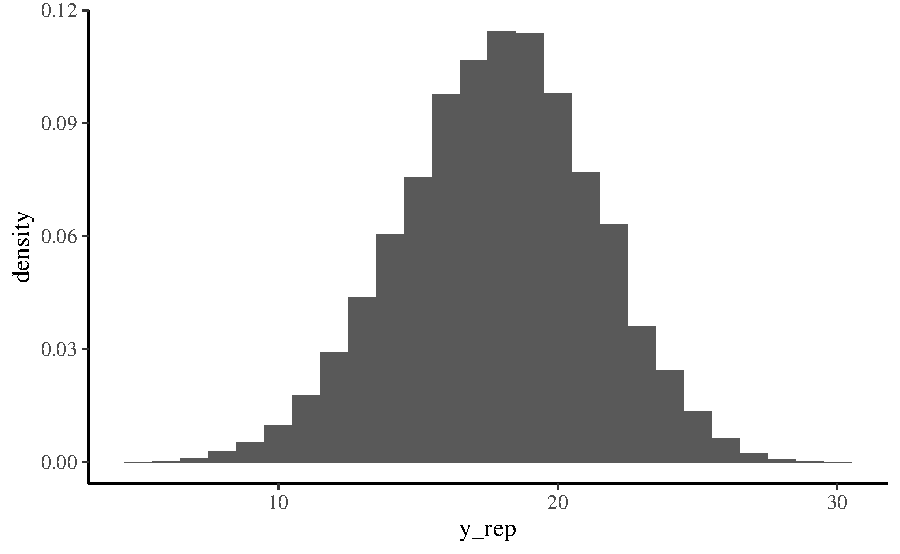
\includegraphics{026_distr_coniugate_files/figure-latex/unnamed-chunk-13-1} \end{center}

\end{example}

\hypertarget{principali-distribuzioni-coniugate}{%
\section{Principali distribuzioni coniugate}\label{principali-distribuzioni-coniugate}}

Esistono molte altre combinazioni simili di verosimiglianza e distribuzione a priori le quali producono una distribuzione a posteriori che ha la stessa densità della distribuzione a priori. Sono elencate qui sotto le più note coniugazioni tra modelli statistici e distribuzioni a priori.

\begin{itemize}
\item
  Per il modello Normale-Normale \(\mathcal{N}(\mu, \sigma^2_0)\), la distribizione iniziale è \(\mathcal{N}(\mu_0, \tau^2)\) e la distribuzione finale è \(\mathcal{N}\left(\frac{\mu_0\sigma^2 + \bar{y}n\tau^2}{\sigma^2 + n\tau^2}, \frac{\sigma^2\tau^2}{\sigma^2 + n\tau^2} \right)\).
\item
  Per il modello Poisson-gamma \(\text{Po}(\theta)\), la distribizione iniziale è \(\Gamma(\lambda, \delta)\) e la distribuzione finale è \(\Gamma(\lambda + n \bar{y}, \delta +n)\).
\item
  Per il modello esponenziale \(\text{Exp}(\theta)\), la distribizione iniziale è \(\Gamma(\lambda, \delta)\) e la distribuzione finale è \(\Gamma(\lambda + n, \delta +n\bar{y})\).
\item
  Per il modello uniforme-Pareto \(\text{U}(0, \theta)\), la distribizione iniziale è \(\text{Pa}(\alpha, \varepsilon)\) e la distribuzione finale è \(\text{Pa}(\alpha + n, \max(y_{(n)}, \varepsilon))\).
\end{itemize}

\hypertarget{considerazioni-conclusive}{%
\section*{Considerazioni conclusive}\label{considerazioni-conclusive}}
\addcontentsline{toc}{section}{Considerazioni conclusive}

Lo scopo di questa discussione è stato quello di mostrare come sia possibile combinare le nostre conoscenze a priori (espresse nei termini di una densità di probabilità) con le evidenze fornite dai dati (espresse nei termini della funzione di verosimiglianza), così da determinare, mediante il teorema di Bayes, una distribuzione a posteriori, la quale condensa l'incertezza che si ha sul parametro \(\theta\). Per illustrare tale problema, abbiamo considerato una situazione nella quale \(\theta\) corrisponde alla probabilità di successo in una sequenza di prove Bernoulliane. Abbiamo visto come, in queste circostanze, è ragionevole esprimere le nostre credenze a priori mediante la densità Beta, con opportuni parametri. L'inferenza rispetto ad una proporzione rappresenta un caso particolare, ovvero un caso nel quale la distribuzione a priori è Beta e la verosimiglianza è Binomiale. In tali circostanze, la distribuzione a posteriori sarà una distribuzione Beta. Per questa ragione, in questo caso specifico, i parametri della distribuzione a posteriori possono essere determinati analiticamente.

\hypertarget{appendix-appendix}{%
\appendix}


  \bibliography{refs.bib,book.bib,packages.bib}

\end{document}
